% !TeX program = xelatex

\documentclass[12pt]{article}
\usepackage{fontspec}
\usepackage{xcolor}
\usepackage{booktabs}
\usepackage{array, multirow, caption}
\usepackage{graphicx}
\graphicspath{ {./Resources/} }
\setmainfont{Linux Libertine O}
\setlength{\parindent}{0em}
\setlength{\parskip}{1em}

\definecolor{light-gray}{gray}{0.89}
\definecolor{lighter-gray}{gray}{0.95}

%usage: example, gloss, translation.
\newcommand{\example}[3]{
	\colorbox{light-gray}{
		\parbox{5in}{
			\emph{Ex.: #1}\\
				  \emph{#2}\\
				  #3
		  }
	}
}

\newcommand{\phrase}[3]{
	\colorbox{lighter-gray}{
		\parbox{2in}{
			\emph{Ex.: #1}\\
				  #2
		  }
	}
}

\newcommand{\word}[1]{
	\emph{#1}
}

\newcommand{\tworow}[1]{
	\multirow{2}{*}{#1}
}

\begin{document}
	\title{Adellian}
	\author{quantumFeline}
	\maketitle

	\tableofcontents

	\section{Phonology}
	
	\begin{tabular} { c c }

		\begin{tabular}{||c | c c c c c c ||}
			\hline
			Consonants & L & A & P-A & P & V & G \\
			\hline
			Nasals & m & \multicolumn{2}{c}{n} & ɲ & & \\
			\tworow{Stops} & \tworow{p} & d & d̠ʒ & ɟ & \tworow{k} & \\
			& & t & t̠ʃ & c & & \\
			\tworow{Continuants} & \tworow{ʋ} & s & ʃ & ç & & \tworow{h} \\
			& & z & ʒ & j & & \\
			Liquids & & l r & & & ʟ & \\
			\hline
		\end{tabular}
		
		&
	
		\begin{tabular}{|| c c c c c || }
			\hline
			ɪ & ɛ & a & ɔ & ʊ \\
			iː & eɪ & aɪ & oʊ & uː \\
			\hline
		\end{tabular}
	
	\end{tabular}
	
	Romanisation:
	
	\begin{tabular} { c c }

		\begin{tabular}{||c | c c c c c c ||}
			\hline
			Consonants & L & A & P-A & P & V & G \\
			\hline
			Nasals & m & \multicolumn{2}{c}{n} & ň & & \\
			\tworow{Stops} & \tworow{p} & d & j & g & \tworow{k} & \\
			& & t & č & c & & \\
			\tworow{Continuants} & \tworow{v} & s & š & x & & \tworow{h} \\
			& & z & ž & y & & \\
			Liquids & & l r & & & w & \\
			\hline
		\end{tabular}
		
		&
	
		\begin{tabular}{|| c c c c c || }
			\hline
			i & e & a & o & u \\
			ii & ei & ai & ou & uu \\
			\hline
		\end{tabular}
	
	\end{tabular}

	\section{Nouns}

	Nouns in Addelian have two genders - animate and inanimate. It influences the pronouns and declensions used for them.
	
	\subsection{Pronouns}
	
	\begin{figure}[h]
	\centering
	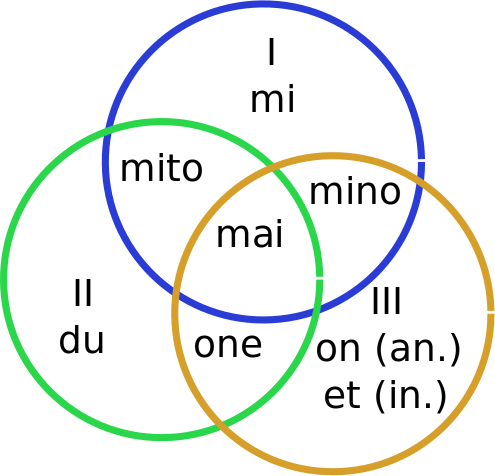
\includegraphics[scale=0.3]{pronouns}
	\caption{Basic Adellian pronouns}
	\end{figure}

	TODO: colour-based pronouns	
	
	Pronouns can also serve as a placeholder when a word root is needed grammatically, but isn't present, meaning-wise.

	Demonstratives are distinguished by three degrees of proximity.

	\begin{tabular}{|| c | c | c ||}
		\hline
		Proximal & Medial & Distal \\
		\hline
		tes & tiis &  navai \\
		\hline
	\end{tabular}
	
	\subsection{Articles}
	
	Adellian has two articles: \word{e[l]} for "a/some", to emphasize that the object discussed is not specific, just that there's some; and \word{an[a]} for "any/in general", to talk about abstractions. By default, no article is used; that indicates definiteness - a specific object discussed.
	There's also a for of the indefinite article \word{ňe[l]} - "no".
	
	\example{Kass šewtal topuki.}
	{cat.AG sit.CONT table.SET.on}
	{The cat is sitting on the table.}
	
	\example{Ňe kass šewtal topuki.}
	{cat.AG.NIND sit.CONT table.SET.on}
	{There's no cat sitting on the table.}
	
	\example{Ana kass šewteli topuki.}
	{cat.AG.GEN sit.HAB table.SET.on}
	{Cats tend to sit on the tables.}
	
	\subsection{Numbers}
	
	The main number forms in Adellian are singular and plural. There is also a dual form, that is used for objects that normally come in pairs, e.g. body parts like arms, items like earrings, etc. It is also used for people and animals to indirectly call them a couple.
	
	Dual and plural for can be combined in the context where it's reasonable to count specifically in pairs.
	
	\begin{tabular}{c c}
	
	\phrase{Oko}{Eye}
	
	&
	
	\phrase{Okoda lidov}{Eyes of a person}
	
	\\
	\rule{0pt}{5ex} 
	
	\phrase{Okos koušoxov}{[Many] eyes of a monster}
	
	&
	
	\phrase{Okodas lidsov}{Eyes of the people}
	
	\end{tabular}
	
	\subsection{Cases}

\end{document}